\part*{Capítulo 8}

\section{Movimiento de tierra}
\begin{itemize}
    \item Desmalezar el terreno
    \item Remover estructuras y árboles existentes
    \item Nivelar el terreno
    \item Señalizar las obras y colocar protecciones
    \item Planificar la circulación de vehículos, maquinarias y personas
    \item Planificar el retiro de escombros
    \item Proteger estructuras y árboles existentes
    \item Determinar las técnicas a emplear para la evacuación de agua subterránea o de superficie
    \item Precauciones especiales con el medio ambiente
\end{itemize}

Antes de iniciar cualquier obra, es necesario replantear los planos en el terreno, marcando referencias que permitan verificar distancias, cotas y ángulos durante la excavación y construcción. Tras las excavaciones, se debe verificar nuevamente el replanteo. En grandes movimientos de tierra, se recomienda escarificar la capa superficial (10 a 20 cm) y almacenarla para reutilizarla. Esto evita la importación de material y ayuda a recuperar semillas y microorganismos locales, favoreciendo un equilibrio ambiental más rápido.

Una excavación puede hacerse empleando variadas técnicas, según las condiciones del proyecto y las restricciones específicas. Algunas son:
\begin{itemize}
    \item Tipo de proyecto de ingeniería.
    \item Tamaño y profundidad de la excavación.
    \item Tipo de terreno (roca o suelo, tipo de estratificación, etc.).
    \item Calidad del suelo (inclinación de taludes o protecciones).
    \item Estructuras contiguas.
    \item Restricciones de espacio.
    \item Equipo y maquinaria disponible.
    \item Presencia de agua subterránea o superficial.
    \item Condiciones ambientales.
\end{itemize}

En trabajos pequeños y en suelo blando, la tierra se puede excavar con palas y picota si se requiere. En excavaciones abiertas con volúmenes mayores de movimiento de tierra se debe considerar el empleo de equipos especializados, como:
\begin{itemize}
    \item Palas Mecánicas: cargadores frontales, retroexcavadoras, palas frontales.
    \item Dragas.
    \item Grúas con cucharón de almeja.
    \item Zanjadoras y otros.
\end{itemize}

\begin{itemize}
    \item \textbf{Excavación de zapata}: Excavación de dimensiones similares (largo, ancho y profundidad).
    \item \textbf{Excavación en zanja}: Excavación larga y angosta (ancho entre 0.5 m y 3.2 m) para fundaciones corridas o canalizaciones.
    \item \textbf{Excavaciones amplias}: Excavaciones de más de 3.2 m de ancho, usadas para subterráneos y grandes fundaciones.
    \item \textbf{Pozos}: Excavaciones profundas y de forma rectangular o circular, para captación de agua o prospección de suelos.
\end{itemize}

Una excavación abierta se puede diseñar de las siguientes formas:
\begin{itemize}
    \item \textbf{Taludes libres}: vertical, inclinado, escalonado.
    \item \textbf{Taludes protegidos}: apuntalados, entibados.
\end{itemize}

Los factores y condiciones especiales de la obra que lo condicionan son:
\begin{itemize}
    \item Tipo de terreno.
    \item Costo relativo entre ambas soluciones.
\end{itemize}

Los factores que condicionan la excavación son:
\begin{itemize}
    \item \textbf{Tiempo de apertura}: Si es prolongado, es recomendable proteger los taludes, especialmente en zonas sísmicas o con vibraciones.
    \item \textbf{Asentamientos permisibles} alrededor de la excavación.
    \item \textbf{Presencia de agua}.
\end{itemize}

\subsubsection{Recomendaciones de talud libre}

\begin{figure}[h]
    \centering
    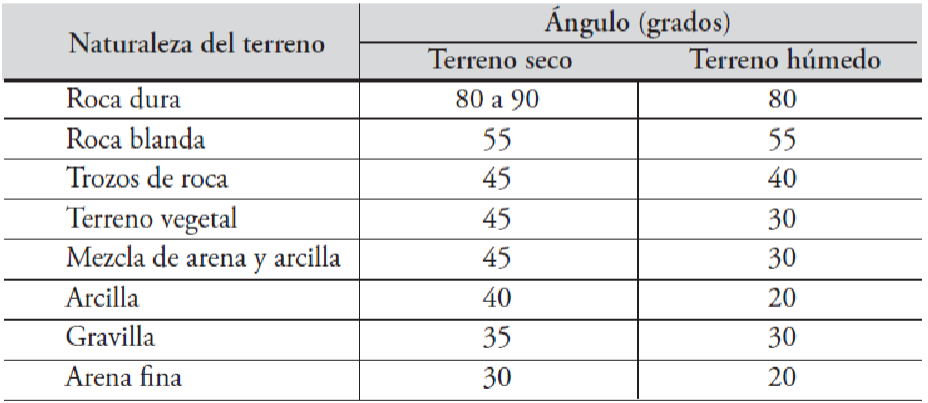
\includegraphics[width=0.8\textwidth]{aaa.png}
    \caption{Recomendaciones de talud libre.}
    \label{fig:8_1}
\end{figure} 

\textbf{Excavaciones con talud libre}: Para excavaciones mayores a 1.2 m de profundidad, si el terreno es cohesivo y permite un talud vertical, se puede realizar sin entibación si se ha calculado la altura crítica de excavación (Hc). La ecuación para Hc es:

\[
Hc = 1.3 \frac{q_u}{\gamma}
\]

donde:
\begin{itemize}
    \item $qu$: resistencia al corte de una muestra de suelo, en kg/m².
    \item $\gamma$: densidad natural del terreno, en kg/m³.
\end{itemize}

Esta fórmula es válida si cualquier sobrecarga en el borde de la excavación está a una distancia mayor que la profundidad de la excavación (Hs).

La altura máxima de excavación, denominada altura de seguridad ($H_s$), se calcula dividiendo la altura crítica $H_c$ por un factor de seguridad (F.S.) entre 1.1 y 2.0:

\[
H_s = \frac{H_c}{F.S.}
\]

Si hay sobrecargas en el borde de la excavación (maquinaria, materiales, etc.), se usará esta fórmula para calcular $H_s$.
